% Regression analysis o state estimation?
\section{Estimación de estado}
La estimación de estado consiste en determinar el estado no medible de un sistema dinámico a partir de las mediciones de entrada y salida de dicho sistema. Lamentablemente, las mediciones no son perfectas, lo que conduce a una inexactitud inherente en el valor de la medición. Para tener en cuenta estos errores, la estimación de estado procesa todas las mediciones disponibles y utiliza un \textit{análisis de regresión} para identificar el estado real probable del sistema.

El análisis de regresión es un análisis estadístico para predecir el valor de una variable cuantitativa. Basándose en un conjunto de variables independientes, se busca estimar la relación de las mismas con una variable dependiente, mediante la obtención de una curva que mejor se ajuste a los datos disponibles, sin que necesariamente pase por todos ellos. En concreto, el modelo de regresión puede representarse como
\begin{equation}
    \textbf{y}_i = f(\textbf{x}_i; \bm{\beta}) + v_i,
    \label{eq:regressionmodel}
\end{equation}
donde la variable $\bm{y}_i$ corresponde a la respuesta o medición para el caso $i$, con $i = 1, 2, ..., m$, $\bm{x_i} = (x_{i1}, x_{i2}, ..., x_{in})$ corresponde al conjunto de valores, fijos o aleatorios, utilizados para explicar o predecir el comportamiento de $y_i$, conocidos como las \textit{variables regresivas} o independientes, $\bm{\beta} = (\beta_1, \beta_2, ..., \beta_n)$ a los parámetros desconocidos\footnote{A diferencia de un estado, el que se define como una magnitud física que varía a través del tiempo, el parámetro es constante a través del tiempo.} a estimar, y $v_i$ a la componente de ruido propia para ese caso.

En base a esto, lo que se busca es estimar la función $f$ que mejor se ajuste a los datos, conocida como \textit{función de expectativa} para el modelo de regresión. Para ello, primero lo que debe hacerse es determinar la forma de dicha función. En base a la forma que adquiera la misma, se puede clasificar en \textit{regresión lineal} y \textit{regresión no lineal}.

% En cambio, cuando la función que modela al sistema \textit{no puede expresarse como una combinación lineal de los parámetros desconocidos} $\bm{\beta}$, se trata entonces de una regresión no lineal, y debe realizarse un proceso iterativo para encontrar la curva que mejor se adapte al sistema.

% La información de tales relaciones se efectúa a partir de información muestral acerca de los valores tomados por $y$, $x_1$, $x_2$, $x_3$, ..., $x_n$, y trata de cuantificar la magnitud de la dependencia entre ellas.

\subsection{Regresión lineal}
En regresión lineal, la variable $y$ \textit{es una combinación lineal} de los parámetros, es decir,
\begin{align}
    y_i &= \beta_1 x_{i1} + \beta_2 x_{i2} + \beta_3 x_{i3} + ... + \beta_n x_{in} + v_i \\
      &= \textbf{x}_i \bm{\beta} + v_i
\end{align}

Existen diferentes métodos dentro del análisis de regresión para poder estimar los parámetros desconocidos $\beta$, siendo uno de los más utilizados el \textit{método de cuadrados mínimos}, el cual plantea que el valor más probable de los parámetros desconocidos será aquel que minimiza la suma de los errores cuadráticos entre lo que se observa y lo que se espera.

\subsubsection{Cuadrados mínimos ordinarios}
Si se quiere, por ejemplo, medir el peso de una bolsa de naranjas, cuyo valor real es $x$, con el uso de una balanza de poca precisión, el valor medido $y$ puede modelarse como el valor real corrompido por ruido, $v$, linealmente mediante la ecuación
\begin{equation}
    y = x + v
    \label{eq:linearmeasmodel}
\end{equation}

Para cada una de las mediciones, se define un término escalar de ruido que es independiente de los otros términos de error ya que, para este caso, se asume que el ruido es independiente y de distribución uniforme. Ahora, si se define el error entre cada medición y el valor verdadero de la bolsa de naranjas, se obtiene el denominado \textit{criterio de error} de cada medición, esto es,
\begin{equation}
    e_i = y_i - x
\end{equation}

Con estos errores definidos, el método de cuadrados mínimos define que la mejor estimación del valor $x$ es la que minimiza el \textit{criterio de error cuadrático},
\begin{equation}
    \hat{x}_{LS} = argmin_x(e_1^2+e_2^2+e_3^2+e_4^2+e_5^2) = \mathscr{L}_{LS}(x),
\end{equation}
aunque a veces también llamada \textit{función de coste de error cuadrático} o \textit{función de pérdida}.

% Luego de un set de cinco mediciones realizadas por separado y en forma secuencial, se obtienen los valores que se observan en la Tabla \ref{tab:naranjasbalanza}, junto con sus modelos de medición y errores cuadráticos.

% \begin{table}[]
\centering
\begin{tabular}{c|c|c|c}
\textbf{Medición} & \textbf{Peso {[}g{]}} & \textbf{Modelo de medición} & \textbf{Error} \\ \hline
1                       & 1012                  & $y_1 = x + v_1$        & $e_1 = y_1 - x$      \\ \hline
2                       & 989                   & $y_2 = x + v_2$        & $e_2 = y_2 - x$      \\ \hline
3                       & 1008                  & $y_3 = x + v_3$        & $e_3 = y_3 - x$      \\ \hline
4                       & 1030                  & $y_4 = x + v_4$        & $e_4 = y_4 - x$      \\ \hline
5                       & 971                   & $y_5 = x + v_5$        & $e_5 = y_5 - x$           
\end{tabular}
\caption{Peso de una bolsa de naranjas para cada medición realizada}
\label{tab:naranjasbalanza}
\end{table}

Para poder minimizar la función de coste, suponiendo que fueron tomadas cinco mediciones realizadas por separado y en forma secuencial, primero hay que reescribir a la función de error en su forma matricial, siendo entonces
\begin{align}
    \textbf{e} &= \textbf{y} - \textbf{H}\cdot x \\
    \begin{bmatrix}
        e_1\\ e_2\\ e_3\\ e_4\\ e_5
    \end{bmatrix}
    &= 
    \begin{bmatrix}
        y_1\\ y_2\\ y_3\\ y_4\\ y_5
    \end{bmatrix}
    -
    \begin{bmatrix}
        1\\ 1\\ 1\\ 1\\ 1
    \end{bmatrix}
    x
\end{align}
siendo \textbf{H} la \textit{matriz Jacobiana}. Dicha matriz tiene las dimensiones de \textit{mxn}, donde \textit{m} es el número de mediciones y \textit{n} es el número de parámetros que se desean estimar. Por ello, \textit{x} si bien en este caso es un escalar, puede ser un vector en el caso que se tengan múltiples indeterminaciones. En base a esto, se puede redefinir a la función de costo como

\begin{align}
    \mathscr{L}_{LS}(x) &= \textbf{e}^T\textbf{e} \\
                        &= (\textbf{y} - \textbf{H}x)^T(\textbf{y} - \textbf{H}x) \\
                        &= \textbf{y}^T\textbf{y} - x^T\textbf{H}^T\textbf{y} - \textbf{y}^T\textbf{H}x + x^T\textbf{H}^T\textbf{H}x
\end{align}

Para minimizar esta ecuación, se procede a computar la derivada parcial de la función de costo respecto a la incertidumbre $x$ para luego igualarla a cero.
\begin{align}
    \frac{\partial \mathscr{L}}{\partial x}\bigg\rvert_{x=\hat{x}} = -\textbf{y}^T\textbf{H} - \textbf{y}^T\textbf{H} + 2\hat{x}^T\textbf{H}^T\textbf{H} &= 0 \\
    -2\textbf{y}^T\textbf{H} + 2\hat{x}^T\textbf{H}^T\textbf{H} &= 0
\end{align}

Despejando, se llega al valor del peso de la bolsa de naranjas que minimiza el criterio de error cuadrático
\begin{equation}
    \hat{x}_{LS} = (\textbf{H}^T\textbf{H})^{-1}\textbf{H}^T\textbf{y}
\end{equation}

Esta expresión tiene solución si y solo si existe $(\textbf{H}^T\textbf{H})^{-1}$, o sea, si la matriz tiene inversa. Si tenemos \textit{m} mediciones y \textit{n} parámetros,
\begin{align*}
    \textbf{H} &\in \Re^{mxn} \\
    \textbf{H}^T\textbf{H} &\in \Re^{nxn}
\end{align*}

Por lo tanto, para que $(\textbf{H}^T\textbf{H})^{-1}$ exista es necesario que se dispongan mínimamente de la misma cantidad de mediciones que variables a estimar, esto es
\begin{equation*}
    m \geq n
\end{equation*}

\subsubsection{Cuadrados mínimos ponderados}

Volviendo al ejemplo de la bolsa de naranjas, si se toman mediciones con distintas balanzas, es lógico pensar que mientras mayor sea la precisión de cada una, mayor importancia tendrá su valor indicado para determinar el peso de la bolsa. Si se considera al modelo de medición lineal con \textit{m} mediciones y \textit{n} incertidumbres,
\begin{align}
    \begin{bmatrix}
        y_1 \\ . \\ . \\ . \\ y_m
    \end{bmatrix}
    &=
    \textbf{H}
    \begin{bmatrix}
        x_1 \\ . \\ . \\ . \\ x_n
    \end{bmatrix}
    +
    \begin{bmatrix}
        v_1 \\ .\\ . \\ . \\ v_m
    \end{bmatrix} \\
    \textbf{y} &= \textbf{H} \textbf{x} + \textbf{v}
\end{align}

En cuadrados mínimos ordinarios, se asume implícitamente que cada término de error, $v_i$, posee el mismo desvío estándar, $\sigma$. En cambio, si se toma que cada término de error es independiente pero con distinto desvío estándar,
\begin{equation}
    \textbf{R} = \mathbb{E}_{[v_i^2]} = \sigma_i^2 \hspace{0.5cm}(i=1,...,m)\hspace{1cm}\textbf{R}=\mathbb{E}_{[\textbf{v}\textbf{v}^T]} = 
    \begin{bmatrix}
        \sigma_1^2  &        &     0      \\
                    & \ddots &            \\
            0       &        & \sigma_m^2
    \end{bmatrix}
\end{equation}

se puede definir a partir de esto el \textit{criterio de cuadrados mínimos ponderados} como
\begin{align}
    \mathscr{L}_{WLS}(x) &= \textbf{e}^T\textbf{R}^{-1}\textbf{e} \\
                         &= \frac{e_1^2}{\sigma_1^2} + \frac{e_2^2}{\sigma_2^2} + ... + \frac{e_m^2}{\sigma_m^2}
\end{align}

Mientras mayor sea el ruido esperado, menor será el peso que tenga en la medición. En el caso que todos los desvíos sean iguales, \textit{no afecta el valor estimado final}, ya que pasa a ser una constante dividiendo a todos los errores.

Expandiendo el nuevo criterio,
\begin{align}
    \mathscr{L}_{WLS}(x) &= \textbf{e}^T\textbf{R}^{-1}\textbf{e} \\
                         &= (\textbf{y} - \textbf{H}\textbf{x})^T\textbf{R}^{-1}(\textbf{y}-\textbf{H}\textbf{x})
\end{align}

Como en el caso de los cuadrados mínimos ordinarios, la ecuación MONGO puede minimizarse realizando el gradiente en este caso al ser que se cuentan con \textit{n} incógnitas.
\begin{equation}
    \frac{\partial \mathscr{L}}{\partial \textbf{x}}\bigg\rvert_{\textbf{x}=\hat{\textbf{x}}} = -\textbf{y}^T\textbf{R}^{-1}\textbf{H} + \hat{\textbf{x}}^T\textbf{H}^T\textbf{R}^{-1}\textbf{H} = 0
\end{equation}

obteniendo entonces las ecuaciones normales ponderadas
\begin{equation}
    \hat{\textbf{x}}_{WLS} = (\textbf{H}^T\textbf{R}^{-1}\textbf{H})^{-1} \textbf{H}^T\textbf{R}^{-1}\textbf{y}
\end{equation}

\subsubsection{Cuadrados mínimos recursivos}

Hasta el momento, todos los datos de las mediciones se encontraban disponibles. Ahora, si lo que se tiene es, por ejemplo, un sensor que entrega datos cada cierto tiempo, con el razonamiento utilizado hasta el momento se tendería a pensar que es necesario correr alguno de los métodos vistos cada vez que llega un dato nuevo con todo el set completo. Se puede apreciar que claramente esto produciría un aumento de costo computacional a medida que transcurre el tiempo, haciendo que en un punto llegue a ser un problema.

Para evitar este problema, lo que se busca es un método recursivo que mantenga un estimador actual del parámetro óptimo para todas las mediciones que se han recolectado hasta ese momento, y luego actualizar dicho estimador dada la medición en el intervalo de tiempo actual. Para lograr esto, se puede utilizar entonces un \textit{estimador lineal recursivo}.

Suponiendo que se tiene un estimador óptimo $\hat{\textbf{x}}_{k-1}$ de los parámetros desconocidos en el tiempo $k-1$ con ruido blanco Gaussiano aditivo. Al llegar la nueva medición en el tiempo $k$,
\begin{equation}
    \textbf{y}_k = \textbf{H}_k \textbf{x} + \textbf{v}_k
\end{equation}

Por lo tanto, el objetivo es poder computar $\hat{\textbf{x}}_k$ como una función de $\textbf{y}_k$ y $\hat{\textbf{x}}_{k-1}$.

Un estimador lineal recursivo está dado por
\begin{equation}
    \hat{\textbf{x}}_k = \hat{\textbf{x}}_{k-1} + \textbf{K}_k (\textbf{y}_k - \textbf{H}_k \hat{\textbf{x}}_{k-1})
\end{equation}

donde $\textbf{K}_k$ es una matriz de ganancia del estimador, el término entre paréntesis se denomina la innovación, y cuantifica que tan bien la medición actual se equipara con el mejor estimador previo. Aún sin conocer la matriz $\textbf{K}_k$, en dicha ecuación puede observarse que el nuevo estimador es la suma del estimador anterior y el término correctivo basado en la diferencia entre lo esperado de la medición y lo que acutalmente se midió. Si la innovación fuese igual a cero, se mantendría el estimador anterior.

Finalmente, para el término $\textbf{K}_k$, lo que se busca es minimizar el \textit{valor esperado de la suma de errores cuadráticos} del estimador actual en el tiempo \textit{k}. Para un solo parámetro escalar,
\begin{align}
    \mathscr{L}_{RLS}(x) &= \mathbb{E}_{[(x_k - \hat{x}_k)^2]} \\
                         &= \sigma_k^2
\end{align}

En cambio, si se tienen \textit{n} parámetros desconocidos en el tiempo \textit{k}
\begin{align}
    \mathscr{L}_{RLS}(x) &= \mathbb{E}_{[(x_{1k} - \hat{x}_{1k})^2 + ... + (x_{nk} - \hat{x}_{nk})^2]} \\
                         &= tr(\textbf{P}_k)
\end{align}

siendo $tr()$ la \textit{traza} (o \textit{trace})\footnote{Corresponde a la suma de los elementos de la diagonal principal de la matriz} de la matriz de covarianza $\textbf{P}_k$. En lugar de minimizar directamente el error, lo que se minimiza es su valor esperado, el cual es la varianza del estimador. A menor varianza, mayor será el grado de confianza del estimador.

Al igual que antes, es posible expresar a la covarianza en función de $\textbf{K}_k$ utilizando la formulación lineal recursiva
\begin{equation}
    \textbf{P}_k = (\textbf{1} - \textbf{K}_k\textbf{H}_k)\textbf{P}_{k-1}(\textbf{1}-\textbf{K}_k\textbf{H}_k)^T + \textbf{K}_k\textbf{R}_k\textbf{K}_k^T
\end{equation}

Mediante el uso de cálculo matricial y derivadas parciales, se puede llegar a que este término se minimiza cuando
\begin{equation}
    \textbf{K}_k = \textbf{P}_{k-1}\textbf{H}_k^T(\textbf{H}_k\textbf{P}_{k-1}\textbf{H}_k^T + \textbf{R}_k)^{-1}
\end{equation}

En base a esto, es posible reescribir la ecuación de la matriz de covarianza como
\begin{align}
    \textbf{P}_k &= \textbf{P}_{k-1} - \textbf{K}_k\textbf{H}_k\textbf{P}_{k-1} \\
                 &= (\textbf{1} - \textbf{K}_k\textbf{H}_k)\textbf{P}_{k-1}
\end{align}

De este último término se puede observar que cuanto más grande sea la matriz de ganancia \textbf{K}, será más pequeña la nueva covarianza del estimador. Por lo tanto, se puede decir que la covarianza \textit{se encoge} con cada medición.

Resumiendo, el algoritmo de los cuadrados mínimos recursivos consta de tres pasos
\begin{enumerate}
    \item Inicializar los parámetros desconocidos y la matriz de covarianza. Esta predicción inicial, por ejemplo, puede obtenerse a partir de la primer medición que se toma y la covarianza puede venir de especificaciones técnicas.
        \begin{align}
            \hat{\textbf{x}}_0 &= \mathbb{E}_{[\textbf{x}]} \\
            \textbf{P}_0 &= \mathbb{E}_{[(\textbf{x} - \hat{\textbf{x}}_0)(\textbf{x} - \hat{\textbf{x}}_0)^T]}
        \end{align}
    \item Definir el Jacobiano y la matriz de covarianza de la medición
        \begin{equation}
          \textbf{y}_k = \textbf{H}_k\textbf{x}+\textbf{v}_k
        \end{equation}
    \item Actualizar el valor estimado de $\hat{\textbf{x}}_k$ y la covarianza $\textbf{P}_k$
        \begin{align}
            \textbf{K}_k &= \textbf{P}_{k-1}\textbf{H}_k^T(\textbf{H}_k\textbf{P}_{k-1}\textbf{H}_k^T + \textbf{R}_k)^{-1} \\
            \hat{\textbf{x}}_k &= \hat{\textbf{x}}_{k-1} + \textbf{K}_k(\textbf{y}_k - \textbf{H}_k\hat{\textbf{x}}_{k-1}) \\
            \textbf{P}_k &= (\textbf{1} - \textbf{K}_k\textbf{H}_k)\textbf{P}_{k-1}
        \end{align}
\end{enumerate}

\subsubsection{Método de máxima verosimilitud}

En lugar de escribir una pérdida, puede aproximarse el problema de la estimación de parámetros óptimos al buscar qué parámetro hacen que las mediciones obtenidas sean las más probables. En otras palabras, cuál \textit{x} maximiza la probabilidad condicional de \textbf{y}
\begin{equation}
    \hat{x} = argmax_x p(y|x)
\end{equation}

Volviendo al ejemplo de la bolsa de naranjas, si se tienen cuatro posibles valores de dicho peso, como se observa en la Figura \ref{fig:mostlikelyproba}, el valor que maximiza la verosimilitud condicional dada la medición $y_med$ corresponde a $x_b$, ya que es la densidad de probabilidad mayor en la ubicación medida.
\begin{figure}
    \centering
    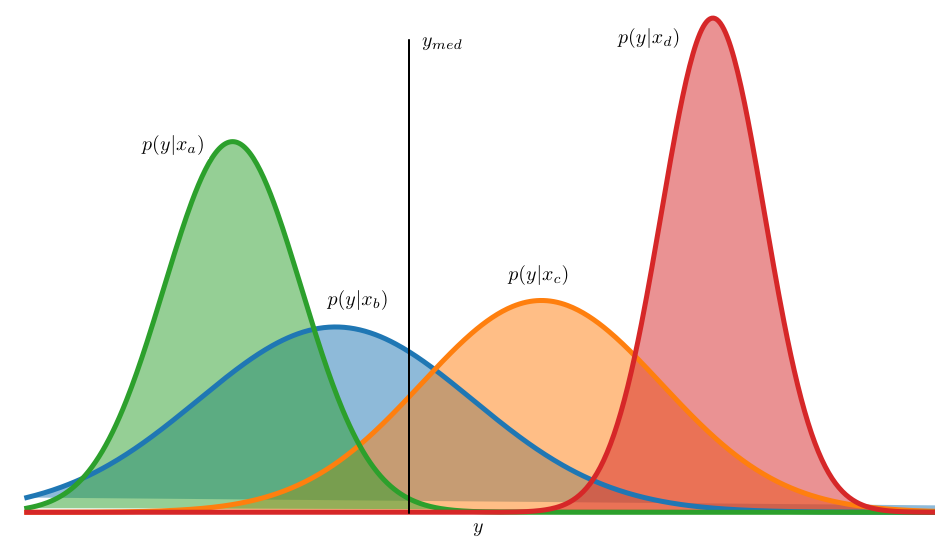
\includegraphics[width=\textwidth]{Img/MostLikelyProba.png}
    \caption{Posibles valores del peso de la bolsa de naranjas y su valor real $y_{med}$}
    \label{fig:mostlikelyproba}
\end{figure}

Tomando en cuenta el modelo de medición presente en la Ecuación \ref{eq:linearmeasmodel}, el mismo puede ser expresado como una probabilidad condicional de la medición, asumiendo alguna densidad de probabilidad para $v$, por ejemplo, ruido blanco Gaussiano aditivo
\begin{equation}
    v \sim \mathcal{N}(0,\sigma^2)
\end{equation}

entonces, el parámetro desconocido, $x$, resulta ser la media de esta densidad, y la varianza corresponde a la varianza de ruido.
\begin{equation}
    p(y|x) = \mathcal{N}(x,\sigma^2)
\end{equation}

Teniendo en cuenta que la función densidad de probabilidad de una Gaussiana es
\begin{equation}
    \mathcal{N}(z;\mu,\sigma^2) = \frac{1}{\sigma \sqrt{2\pi}} e^{\frac{-(z-\mu)^2}{2\sigma^2}}
\end{equation}

puede expresarse la medición de verosimilitud para una de las mediciones como
\begin{align}
    p(y|x) &= \mathscr{N}(y;x,\sigma^2) \\
           &= \frac{1}{\sqrt{2\pi\sigma^2}} e^{\frac{-(y-x)^2}{2\sigma^2}}
\end{align}

Si se tienen múltiples mediciones múltiples independientes, entonces
\begin{align}
    p(\textbf{y}|x) &\propto \mathscr{N}(y_1;x,\sigma^2)\cdot\mathscr{N}(y_2;x,\sigma^2)\cdot...\cdot\mathscr{N}(y_m;x,\sigma^2) \\
            &= \frac{1}{\sqrt{(2\pi)^m\sigma^{2m}}} \exp\left({\frac{-\sum_{i=1}^m(y_i-x)^2}{2\sigma^2}}\right)
\end{align}

El estimador de máxima verosimilitud (MLE) está dado por
\begin{equation}
    \hat{x}_{MLE} = argmax_x p(\textbf{y}|x)
\end{equation}

En lugar de tratar de optimizar el verosímil directamente, puede aplicarse el logaritmo
\begin{align}
    \hat{x}_{MLE} = argmax_x \log p(\textbf{y}|x)
\end{align}

El logaritmo aumenta monotónicamente. Resulta entonces
\begin{equation}
    \log p(\textbf{y}|x) = -\frac{1}{2\sigma^2}\left((y_1-x)^2+...+(y_m-x)^2\right)+C
\end{equation}

Esta ecuación es muy parecida a la suma de los errores cuadráticos. La constante $C$ en esta expresión refiere a términos que no son funciones de $x$ y pueden ser ignorados.

Luego, como el argmax de la función f es equivalente al argmin del negativo de dicha función, 
\begin{equation}
    argmax_z f(z) = argmin_z \left(-f(z)\right)
\end{equation}

el problema del verosímil máximo puede ser escrito como
\begin{align}
    \hat{x}_{MLE} &= argmin_x -\left(\log p(\textbf{y}|x)\right) \\
                  &= argmin_x \frac{1}{2\sigma^2}\left((y_1-x)^2+...+(y_m-x)^2\right)
\end{align}

Por lo tanto, es posible realizar la maximización de la verosimilitud mediante una minimización de la suma de errores cuadráticos. Esto es válido ya que se asume que las mediciones se encuentran corrompidas por ruido blanco Gaussiano independiente aditivo de igual varianza.

Finalmente, si se asume que cada medición tiene una varianza distinta, se llega al mismo criterio que en cuadrados mínimos ponderados
\begin{equation}
    \hat{x}_{MLE} = argmin_x \frac{1}{2}\left(\frac{(y_1-x)^2}{\sigma_1^2}+...+\frac{(y_m-x)^2}{\sigma_m^2}\right)
\end{equation}

Resumiendo, en ambos casos, el estimador de máxima verosimilitud para ruido blanco Gaussiano es equivalente a las soluciones de los cuadrados mínimos ordinarios o ponderados.
\begin{equation}
    \hat{x}_{MLE} = \hat{x}_{LS} = argmin_x\mathscr{L}_{LS}(x) = argmin_x\mathscr{L}_{MLE}(x)
\end{equation}

Esto cobra importancia en sistemas realistas, los cuales presentan una gran cantidad de fuentes de ruido. Recordando el teorema central del límite, que establece que cuando se suman variables aleatorias independientes, su suma normalizada tenedrá a una distribución normal, y teniendo en cuenta que el método de cuadrados mínimos es equivalente a calcular la máxima verosimilitud\footnote{Siempre asumiendo que se está en presencia de ruido blanco Gaussiano aditivo}, es posible calcular el mejor estimador de una forma computacionalmente sencilla.

Sin embargo, una consideración importante a tener en cuenta con el método de cuadrados mínimos es cuando se presenta un valor atípico, esto es, los que se encuentran en las "colas" de la Gaussiana, provocando que el estimador final se aleje del valor verdadero. Por ello es importante cuantificar la distribución de error antes de aplicar ciegamente máxima verosimilitud o cuadrados mínimos.

\subsection{Cuadrados mínimos no lineales}

La regresión lineal es un método poderoso para analizar los datos descriptos por modelos que son lineales en los parámetros. Sin embargo, muchas veces las formas de las curvas que mejor ajustan a los datos obtenidos son no lineales en los parámetros. En estos casos, el modelo de regresión sigue siendo de la misma forma que el de la Ecuación \ref{eq:regressionmodel}, a diferencia de que al menos una de las derivadas de la función de expectativa con respecto a los parámetros depende de al menos uno de los parámetros.

Para diferenciar entre modelos lineales y no lineales, los parámetros para este último caso se definen con $\bm{\theta}$,
\begin{equation}
    y_i = f(\textbf{x}_i, \bm{\theta}) + v_i
    \label{eq:nonlinearregressionmodel}
\end{equation}

